% =====================================================================
\chapter{Códigos de fuente y código de Huffman}
\label{tema:3}
% =====================================================================

Este tema da a la entropía su significado operativo: es la longitud media mínima, en bits por símbolo, de una descripción sin pérdidas de la fuente. Se estudian los códigos prefijo, la desigualdad de Kraft, las cotas para la longitud óptima y el algoritmo de Huffman~\cite{huffman}. Se sigue~\cite[cap.~5]{ct}, en particular §5.1--5.4, §5.6 y §5.8; MacKay~\cite[cap.~5]{mackay} presenta el mismo material con el nombre de \emph{códigos de símbolos}, que es también el enfoque del tema «Source coding and data compression» de~\cite{camit}.

\section{Códigos de símbolos}

\begin{definicion}[Código]\label{def:codigo}
Un \emph{código binario} para una variable $X$ con alfabeto $\X$ es una aplicación $C\colon\X\to\{\bin{0},\bin{1}\}^{*}$ que asigna a cada símbolo una cadena finita de bits, su \emph{palabra de código}, de longitud $\ell(x)$. La \emph{extensión} de $C$ codifica una secuencia concatenando palabras: $C(x_1\cdots x_n)=C(x_1)\cdots C(x_n)$. La \emph{longitud media} del código es $L(C)=\sum_{x}p(x)\,\ell(x)$.
\end{definicion}

\begin{definicion}[Clases de códigos]\label{def:clases}
Un código es
\begin{enumerate}
  \item \emph{no singular} si $C$ es inyectiva;
  \item \emph{unívocamente descodificable} si su extensión es inyectiva, es decir, si toda cadena de bits procede de, a lo sumo, una secuencia de símbolos;
  \item \emph{prefijo} o \emph{instantáneo} si ninguna palabra de código es prefijo de otra distinta.
\end{enumerate}
\end{definicion}

Cada clase contiene a la siguiente: todo código prefijo es unívocamente descodificable, porque el receptor reconoce el final de cada palabra en cuanto la lee completa, sin mirar los bits posteriores; y todo código unívocamente descodificable es no singular.

\begin{ejemplo}\label{ej:clases}
Sea $\X=\{\mathrm{a},\mathrm{b},\mathrm{c},\mathrm{d}\}$. En la tabla siguiente, $C_1$ es singular ($\mathrm{a}$ y $\mathrm{b}$ comparten palabra); $C_2$ es no singular pero no unívocamente descodificable, porque la cadena \bin{010} puede leerse como $\mathrm{b}$, como $\mathrm{ca}$ o como $\mathrm{ad}$; $C_3$ es unívocamente descodificable, porque cada palabra empieza por \bin{0} y basta cortar delante de cada \bin{0}, pero no es prefijo; $C_4$ es prefijo.
\begin{center}
\begin{tabular}{@{}ccccc@{}}
\toprule
$x$ & $C_1$ & $C_2$ & $C_3$ & $C_4$ \\
\midrule
a & \bin{0} & \bin{0} & \bin{0} & \bin{0} \\
b & \bin{0} & \bin{010} & \bin{01} & \bin{10} \\
c & \bin{1} & \bin{01} & \bin{011} & \bin{110} \\
d & \bin{10} & \bin{10} & \bin{0111} & \bin{111} \\
\bottomrule
\end{tabular}
\end{center}
\end{ejemplo}

\section{La desigualdad de Kraft}

A cada cadena binaria $c=c_1\cdots c_\ell$ se le asocia el \emph{intervalo diádico} $J(c)=[0.c_1\cdots c_\ell,\ 0.c_1\cdots c_\ell+2^{-\ell})\subseteq[0,1)$, donde $0.c_1\cdots c_\ell=\sum_{i}c_i2^{-i}$. Es el conjunto de números de $[0,1)$ cuya expansión binaria empieza por $c$, y tiene longitud $2^{-\ell}$. Dos intervalos diádicos están contenidos uno en otro o son disjuntos, y $J(c')\subseteq J(c)$ si y solo si $c$ es prefijo de $c'$.

\begin{teorema}[Desigualdad de Kraft]\label{teo:kraft}
Las longitudes $\ell_1,\dots,\ell_m$ de las palabras de un código binario prefijo cumplen
\[
\sum_{i=1}^{m}2^{-\ell_i}\le 1.
\]
Recíprocamente, si unos enteros positivos $\ell_1,\dots,\ell_m$ cumplen esta desigualdad, existe un código prefijo con esas longitudes.
\end{teorema}

\begin{proof}
Si el código es prefijo, ninguna palabra es prefijo de otra, así que los intervalos $J(c_1),\dots,J(c_m)$ son disjuntos dos a dos. Son subintervalos de $[0,1)$, luego la suma de sus longitudes, $\sum_i2^{-\ell_i}$, no supera~1.

Para el recíproco, se ordenan las longitudes de forma que $\ell_1\le\dots\le\ell_m$ y se define $s_i=\sum_{j<i}2^{-\ell_j}$ (con $s_1=0$). Cada término $2^{-\ell_j}$ con $j<i$ es múltiplo de $2^{-\ell_i}$, porque $\ell_j\le\ell_i$; por tanto $s_i$ se escribe en binario con $\ell_i$ cifras tras la coma, completando con ceros si hace falta,, que se toman como palabra $c_i$, y $J(c_i)=[s_i,s_i+2^{-\ell_i})$. Estos intervalos son consecutivos y disjuntos, y el último termina en $s_m+2^{-\ell_m}=\sum_j2^{-\ell_j}\le 1$. Como son disjuntos, ninguna palabra es prefijo de otra.
\end{proof}

\begin{figure}[h]
\centering
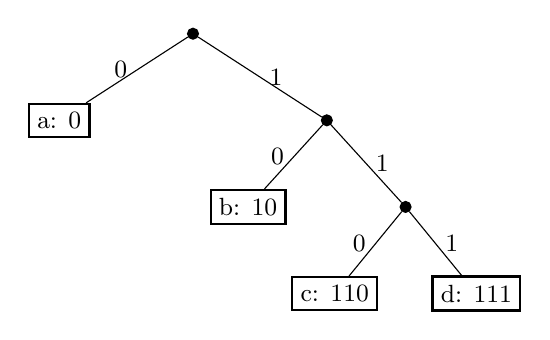
\begin{tikzpicture}[font=\small,
  level distance=11mm,
  level 1/.style={sibling distance=34mm},
  level 2/.style={sibling distance=20mm},
  level 3/.style={sibling distance=18mm},
  nodo/.style={circle,draw,inner sep=1.4pt,fill=black},
  hoja/.style={rectangle,draw,thick,inner sep=3pt}]
  \node[nodo] {}
    child {node[hoja] {a: \bin{0}} edge from parent node[left] {\bin{0}}}
    child {node[nodo] {}
      child {node[hoja] {b: \bin{10}} edge from parent node[left] {\bin{0}}}
      child {node[nodo] {}
        child {node[hoja] {c: \bin{110}} edge from parent node[left] {\bin{0}}}
        child {node[hoja] {d: \bin{111}} edge from parent node[right] {\bin{1}}}
        edge from parent node[right] {\bin{1}}}
      edge from parent node[right] {\bin{1}}};
\end{tikzpicture}
\caption{El código prefijo $C_4$ del \cref{ej:clases} como árbol binario: las palabras son las hojas y ninguna está en el camino hacia otra. La suma de Kraft es $\tfrac12+\tfrac14+\tfrac18+\tfrac18=1$.}
\label{fig:arbol-kraft}
\end{figure}

\begin{observacion}
McMillan demostró que la desigualdad de Kraft la cumplen también todos los códigos unívocamente descodificables~\cite[§5.5]{ct}. Por tanto, restringirse a códigos prefijo no tiene coste: cualquier conjunto de longitudes alcanzable con un código unívocamente descodificable lo es también con uno prefijo.
\end{observacion}

\section{Cotas para la longitud óptima}

\begin{teorema}[Cota inferior]\label{teo:cota-inferior}
La longitud media de todo código prefijo para $X$ cumple $L\ge H(X)$, con igualdad si y solo si $p(x)=2^{-\ell(x)}$ para todo $x$.
\end{teorema}

\begin{proof}
Sea $c=\sum_x2^{-\ell(x)}\le 1$ (\cref{teo:kraft}) y sea $r(x)=2^{-\ell(x)}/c$, que es una distribución. Como $\ell(x)=-\log r(x)-\log c$,
\[
L-H(X)=\sum_x p(x)\ell(x)+\sum_xp(x)\log p(x)=\sum_xp(x)\log\frac{p(x)}{r(x)}-\log c=\KL{p}{r}+\log\frac1c\ge 0,
\]
porque los dos sumandos finales son no negativos (\cref{teo:gibbs} y $c\le 1$). La igualdad exige $c=1$ y $p=r$, es decir, $p(x)=2^{-\ell(x)}$.
\end{proof}

La demostración interpreta cada código prefijo como un modelo probabilístico implícito, $r(x)\propto2^{-\ell(x)}$: un código asigna palabras cortas a lo que «cree» probable. Esta lectura es la mitad de la equivalencia entre predecir y comprimir que se completa en el \cref{tema:4}.

\begin{definicion}[Código de Shannon]\label{def:shannon}
Un \emph{código de Shannon} para $p$ es un código prefijo con longitudes $\ell(x)=\lceil-\log p(x)\rceil$.
\end{definicion}

Estas longitudes cumplen la desigualdad de Kraft, porque $2^{-\lceil-\log p(x)\rceil}\le2^{\log p(x)}=p(x)$ y las $p(x)$ suman~1; por el \cref{teo:kraft}, el código existe.

\begin{teorema}[Longitud óptima]\label{teo:cotas}
Sea $L^{*}$ la mínima longitud media de un código prefijo para $X$. Entonces
\[
H(X)\le L^{*}<H(X)+1.
\]
\end{teorema}

\begin{proof}
La cota inferior es el \cref{teo:cota-inferior}. Para la superior, el código de Shannon cumple $\ell(x)<-\log p(x)+1$, luego $L^{*}\le\sum_xp(x)\ell(x)<\sum_xp(x)\bigl(-\log p(x)+1\bigr)=H(X)+1$~\cite[§5.4]{ct}.
\end{proof}

El exceso de hasta un bit se debe a que las longitudes han de ser enteras. Se reparte entre muchos símbolos codificando bloques.

\begin{corolario}[Codificación por bloques]\label{cor:bloques}
Sean $X_1,\dots,X_n$ independientes y con la misma distribución que $X$, y sea $L_n^{*}$ la longitud media mínima de un código prefijo para el bloque $(X_1,\dots,X_n)$. Entonces
\[
H(X)\le\frac{L_n^{*}}{n}<H(X)+\frac1n.
\]
En particular, $L_n^{*}/n\to H(X)$ cuando $n\to\infty$.
\end{corolario}

\begin{proof}
Por independencia, $H(X_1,\dots,X_n)=nH(X)$ (\cref{cor:cadena-secuencias}). Basta aplicar el \cref{teo:cotas} al bloque y dividir por $n$.
\end{proof}

El \cref{cor:bloques} es una forma del \emph{teorema de codificación de fuente} de Shannon: la entropía es el número mínimo de bits por símbolo con que puede describirse la fuente sin pérdidas, y ese mínimo se alcanza asintóticamente~\cite[cap.~4]{mackay}.

\section{El código de Huffman}

\begin{definicion}[Algoritmo de Huffman]\label{def:huffman}
Dada una distribución sobre $K\ge 2$ símbolos, el \emph{algoritmo de Huffman} construye un árbol binario: mientras quede más de un nodo, fusiona los dos nodos de menor probabilidad en un nodo nuevo cuya probabilidad es la suma de ambas. Al terminar, las ramas que salen de cada nodo se etiquetan con \bin{0} y \bin{1}, y la palabra de cada símbolo es la secuencia de etiquetas desde la raíz hasta su hoja.
\end{definicion}

Cada fusión añade un bit a la palabra de todos los símbolos de los dos nodos fusionados; por eso los símbolos poco probables, que se fusionan pronto, reciben palabras largas.

\begin{ejemplo}\label{ej:huffman}
Sea $p=(0{,}4;\ 0{,}2;\ 0{,}2;\ 0{,}1;\ 0{,}1)$ sobre $\{\mathrm{a},\mathrm{b},\mathrm{c},\mathrm{d},\mathrm{e}\}$. Las fusiones son: $\mathrm{d}+\mathrm{e}\to 0{,}2$; $\mathrm{b}+\mathrm{c}\to 0{,}4$; $\{\mathrm{d},\mathrm{e}\}+\mathrm{a}\to 0{,}6$; y finalmente $0{,}4+0{,}6\to 1$. Resulta el árbol de la \cref{fig:huffman}, con longitud media
\[
L=0{,}4\cdot 2+0{,}2\cdot 2+0{,}2\cdot 2+0{,}1\cdot 3+0{,}1\cdot 3=2{,}2\text{ bits},
\]
frente a $H(p)=2{,}122$ bits y a los 3 bits de un código de longitud fija.
\end{ejemplo}

\begin{figure}[h]
\centering
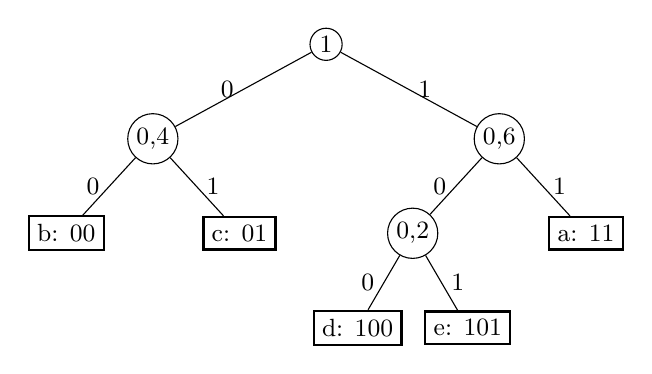
\begin{tikzpicture}[font=\small,
  level distance=12mm,
  level 1/.style={sibling distance=44mm},
  level 2/.style={sibling distance=22mm},
  level 3/.style={sibling distance=14mm},
  nodo/.style={circle,draw,inner sep=1.5pt},
  hoja/.style={rectangle,draw,thick,inner sep=3pt}]
  \node[nodo] {$1$}
    child {node[nodo] {$0{,}4$}
      child {node[hoja] {b: \bin{00}} edge from parent node[left] {\bin{0}}}
      child {node[hoja] {c: \bin{01}} edge from parent node[right] {\bin{1}}}
      edge from parent node[left] {\bin{0}}}
    child {node[nodo] {$0{,}6$}
      child {node[nodo] {$0{,}2$}
        child {node[hoja] {d: \bin{100}} edge from parent node[left] {\bin{0}}}
        child {node[hoja] {e: \bin{101}} edge from parent node[right] {\bin{1}}}
        edge from parent node[left] {\bin{0}}}
      child {node[hoja] {a: \bin{11}} edge from parent node[right] {\bin{1}}}
      edge from parent node[right] {\bin{1}}};
\end{tikzpicture}
\caption{Árbol de Huffman del \cref{ej:huffman}. Cada nodo interno lleva la suma de las probabilidades de sus hojas.}
\label{fig:huffman}
\end{figure}

La optimalidad del algoritmo se apoya en dos propiedades de los códigos óptimos.

\begin{lema}\label{lem:optimo}
Sea $p_1\ge p_2\ge\dots\ge p_K>0$, con $K\ge 2$. Existe un código prefijo óptimo con longitudes $\ell_1,\dots,\ell_K$ tal que
\begin{enumerate}
  \item $\ell_1\le\ell_2\le\dots\le\ell_K$;
  \item las palabras de los dos símbolos menos probables, $K-1$ y $K$, tienen la longitud máxima $\ell_K$ y solo difieren en el último bit.
\end{enumerate}
\end{lema}

\begin{proof}
Existe un código óptimo, porque hay un número finito de asignaciones de longitudes con $L$ menor que la de un código fijo. Sea $C$ uno de ellos. (i) Si $p_j>p_k$ y $\ell_j>\ell_k$, intercambiar las palabras de $j$ y $k$ cambia la longitud media en $(p_j-p_k)(\ell_k-\ell_j)<0$, contra la optimalidad; luego $p_j>p_k$ implica $\ell_j\le\ell_k$. Entre símbolos de igual probabilidad, intercambiar palabras no cambia $L$, así que puede ordenarse para que $\ell_1\le\dots\le\ell_K$. (ii) Sea $w$ una palabra de longitud máxima $\ell_K$ y sea $w'$ la cadena que resulta de cambiar su último bit. Si $w'$ no fuese una palabra del código, podría suprimirse el último bit de $w$: ninguna otra palabra empezaría por la cadena acortada, porque tendría que empezar por $w'$ y no hay palabras más largas que $\ell_K$, y ninguna palabra sería prefijo de ella, porque lo sería también de $w$. El código seguiría siendo prefijo y tendría menor longitud media, contra la optimalidad. Luego $w'$ es una palabra de longitud $\ell_K$. Por último, se asignan $w$ y $w'$ a los símbolos $K$ y $K-1$ intercambiando palabras; si $j\le K-1$ tenía asignada una de ellas, el intercambio de las palabras de $j$ y $K-1$ cambia $L$ en $(p_{K-1}-p_j)(\ell_K-\ell_{K-1})\le 0$, de modo que el código sigue siendo óptimo.
\end{proof}

\begin{teorema}[Optimalidad del código de Huffman]\label{teo:huffman}
El código de Huffman tiene longitud media mínima entre todos los códigos prefijo para $p$.
\end{teorema}

\begin{proof}
Por inducción sobre $K$. Para $K=2$, Huffman asigna \bin{0} y \bin{1}, con $L=1$, que es óptimo. Sea $K\ge 3$ con $p_1\ge\dots\ge p_K$, y sea $p'$ la distribución sobre $K-1$ símbolos que resulta de fusionar $K-1$ y $K$ en uno de probabilidad $p_{K-1}+p_K$; su código de Huffman es el de $p$ con las dos hojas hermanas sustituidas por su padre.

Todo código prefijo $C'$ para $p'$ da un código para $p$ al añadir \bin{0} y \bin{1} a la palabra del símbolo fusionado, con longitud media $L(C')+p_{K-1}+p_K$. Recíprocamente, el código óptimo $C$ del \cref{lem:optimo} da un código para $p'$ al sustituir las dos hojas hermanas por su padre, con longitud media $L(C)-p_{K-1}-p_K$. De ambas construcciones se deduce $L^{*}(p)=L^{*}(p')+p_{K-1}+p_K$. Por la hipótesis de inducción, el código de Huffman de $p'$ es óptimo, y el de $p$ tiene longitud $L^{*}(p')+p_{K-1}+p_K=L^{*}(p)$~\cite[§5.8]{ct}.
\end{proof}

Por los Teoremas~\ref{teo:cotas} y~\ref{teo:huffman}, $H(p)\le L_{\text{Huffman}}<H(p)+1$, con $L_{\text{Huffman}}=H(p)$ cuando todas las probabilidades son potencias de $1/2$. El código óptimo no es único: con otros desempates en el \cref{ej:huffman} se obtiene un árbol distinto (\cref{eje:3-dos-huffman}).

\section{El límite de los códigos de símbolos}

Un código de símbolos gasta un número entero de bits por símbolo, y al menos un bit. Si $p=(0{,}9;\ 0{,}1)$, la entropía es $H_b(0{,}1)=0{,}469$ bits, pero cualquier código de símbolos para dos resultados gasta 1 bit por símbolo: más del doble. La codificación por bloques del \cref{cor:bloques} reduce el exceso, pero un bloque de $n$ símbolos sobre un alfabeto de $K$ símbolos tiene $K^{n}$ valores posibles, y la tabla del código crece exponencialmente.

\begin{observacion}[Conexión con los LLM]
Un modelo de lenguaje asigna con frecuencia probabilidades muy altas al token siguiente: si $q(x_t\mid x_{1:t-1})=0{,}99$, la sorpresa es $-\log 0{,}99=0{,}0145$ bits, y un código de símbolos gastaría al menos un bit para ese token, unas setenta veces más. Además, la distribución cambia en cada posición, de modo que habría que construir un código de Huffman distinto para cada contexto. El \cref{tema:4} presenta un método que gasta, de hecho, fracciones de bit por símbolo y admite un modelo distinto en cada paso: la codificación aritmética.
\end{observacion}

\begin{lecturas}
\item Cover y Thomas~\cite{ct}, §5.1 «Examples of Codes», §5.2 «Kraft Inequality», §5.4 «Bounds on the Optimal Code Length», §5.6 «Huffman Codes» y §5.8 «Optimality of Huffman Codes».
\item MacKay~\cite{mackay}, cap.~5 «Symbol Codes».
\item Huffman~\cite{huffman}, artículo original.
\item Universidad de Cambridge, \emph{Information Theory}~\cite{camit}, tema «Source coding and data compression».
\end{lecturas}

\section*{Ejercicios del tema 3}
\addcontentsline{toc}{section}{Ejercicios del tema 3}

\begin{ejercicio}{1}{eje:3-dos-huffman}
¿Pueden dos personas que aplican correctamente el algoritmo de Huffman a la misma distribución obtener códigos con conjuntos de longitudes distintos? Respóndalo con la distribución del \cref{ej:huffman}, deshaciendo de otra forma el empate de la tercera fusión, y compare las longitudes medias.
\fuente{adaptado de Universidad de Cambridge, \emph{Information Theory}~\cite{camit}, \emph{Examples Sheet}, \emph{Supervision}~1, ejercicio~13.}
\end{ejercicio}

\begin{ejercicio}{2}{eje:3-diadica}
Sea $p=(1/2,1/4,1/8,1/8)$. Calcule $H(p)$, la longitud de un código de longitud fija y un código de Huffman con su longitud media. Compruebe la desigualdad de Kraft.
\end{ejercicio}

\begin{ejercicio}{2}{eje:3-huffman5}
Construya un código de Huffman para $p=(0{,}35;\ 0{,}25;\ 0{,}2;\ 0{,}15;\ 0{,}05)$. Calcule su longitud media y compárela con $H(p)=2{,}121$ bits y con la cota del \cref{teo:cotas}.
\end{ejercicio}

\begin{ejercicio}{2}{eje:3-unica}
Considere el código binario $\{\bin{00},\bin{11},\bin{0101},\bin{111},\bin{1010},\bin{100100},\bin{0110}\}$. ¿Es un código prefijo? ¿Cumplen sus longitudes la desigualdad de Kraft? ¿Es unívocamente descodificable? Si no lo es, dé una cadena ambigua.
\fuente{adaptado de MacKay~\cite{mackay}, ejercicio~5.19, tal como lo propone Universidad de Cambridge, \emph{Information Theory}~\cite{camit}, \emph{Examples Sheet}, \emph{Supervision}~1, ejercicio~10.}
\end{ejercicio}

\begin{ejercicio}{2}{eje:3-shannon}
Para la distribución del \cref{ej:huffman}, calcule las longitudes del código de Shannon, su suma de Kraft y su longitud media. Compruebe que cumple el \cref{teo:cotas} y compárelo con el código de Huffman.
\end{ejercicio}

\begin{ejercicio}{2}{eje:3-bloques}
Una fuente binaria sin memoria emite \bin{a} con probabilidad $0{,}9$ y \bin{b} con probabilidad $0{,}1$. (a) ¿Cuántos bits por símbolo gasta el código de Huffman símbolo a símbolo? (b) Construya el código de Huffman para pares de símbolos y calcule su longitud media por símbolo. (c) Compare con $H_b(0{,}1)$ y con la cota del \cref{cor:bloques} para $n=2$.
\end{ejercicio}

\begin{ejercicio}{3}{eje:3-no-comprime}
Sea $C\colon\{\bin{0},\bin{1}\}^{+}\to\{\bin{0},\bin{1}\}^{+}$ una aplicación inyectiva entre cadenas binarias no vacías (un compresor sin pérdidas). Demuestre que, si $C$ acorta alguna cadena, entonces alarga alguna otra. Indicación: cuente las cadenas de longitud a lo sumo $n$.
\fuente{adaptado de Universidad de Cambridge, \emph{Information Theory}~\cite{camit}, \emph{Examples Sheet}, \emph{Supervision}~2, ejercicio~7.}
\end{ejercicio}
